% !TEX root = ../foresight.tex

\section{Planning For Exploration}

Planning a path to observe the blind spots of an autonomous car is broken into
following steps. First, using the 2D laser scan from the car, the bounding
polygon is computed. This polygon represents the known free space where the
quadrotor can travel. The laser scan is also used to determine regions in space
where that the car is not able to sense. These regions are called blind
regions. Using these blind regions and the bounding polygon, a path is computed
for the quadrotor that maximizes the observed area of the blind regions while
staying within the bounding polygon. The path is computed for a given time
horizon.

The remainder of this section is structured as follows; Sec.~\ref{sec:poly}
introduces the our formal definition of a laser scan and describes how the
bounding polygon is found, Sec.~\ref{sec:blindregions} describes how the blind
regions are computed from the laser scan, and Sec.~\ref{sec:planner} describes
and analyzes the algorithm we developed for computing the exploratory path.

% \begin{figure}
%     \centering
%     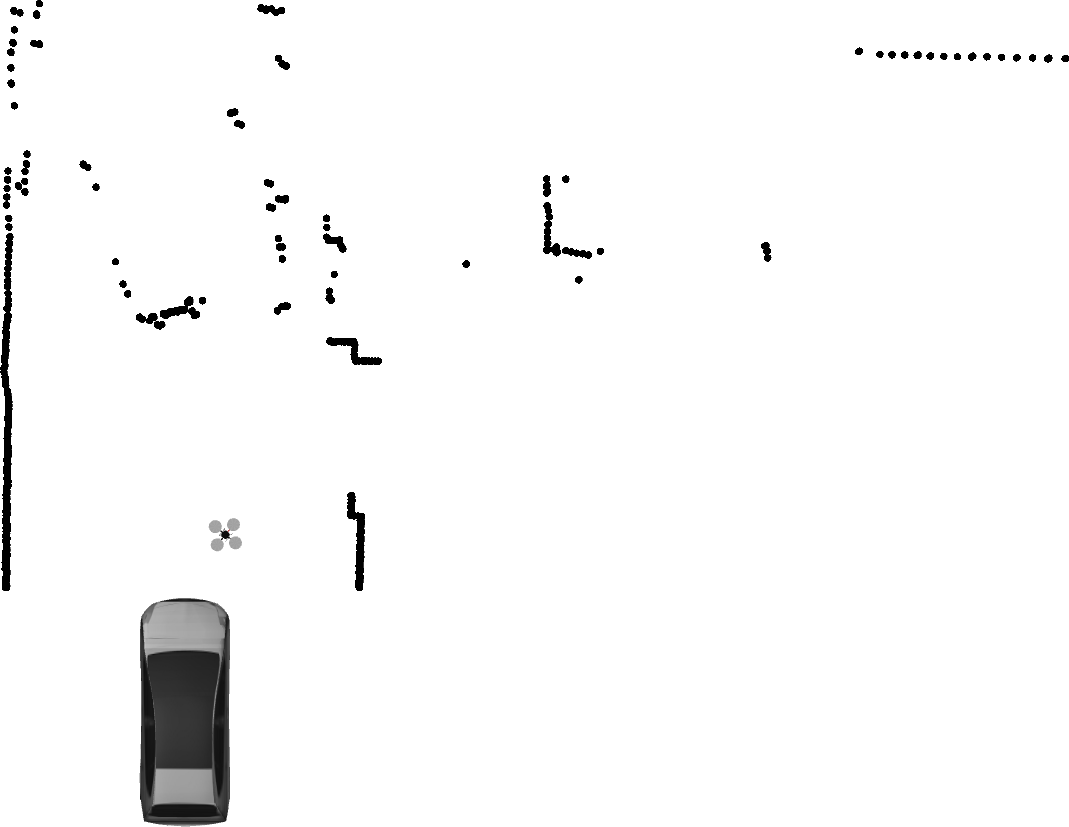
\includegraphics[width=0.49\linewidth]{01laser}
%     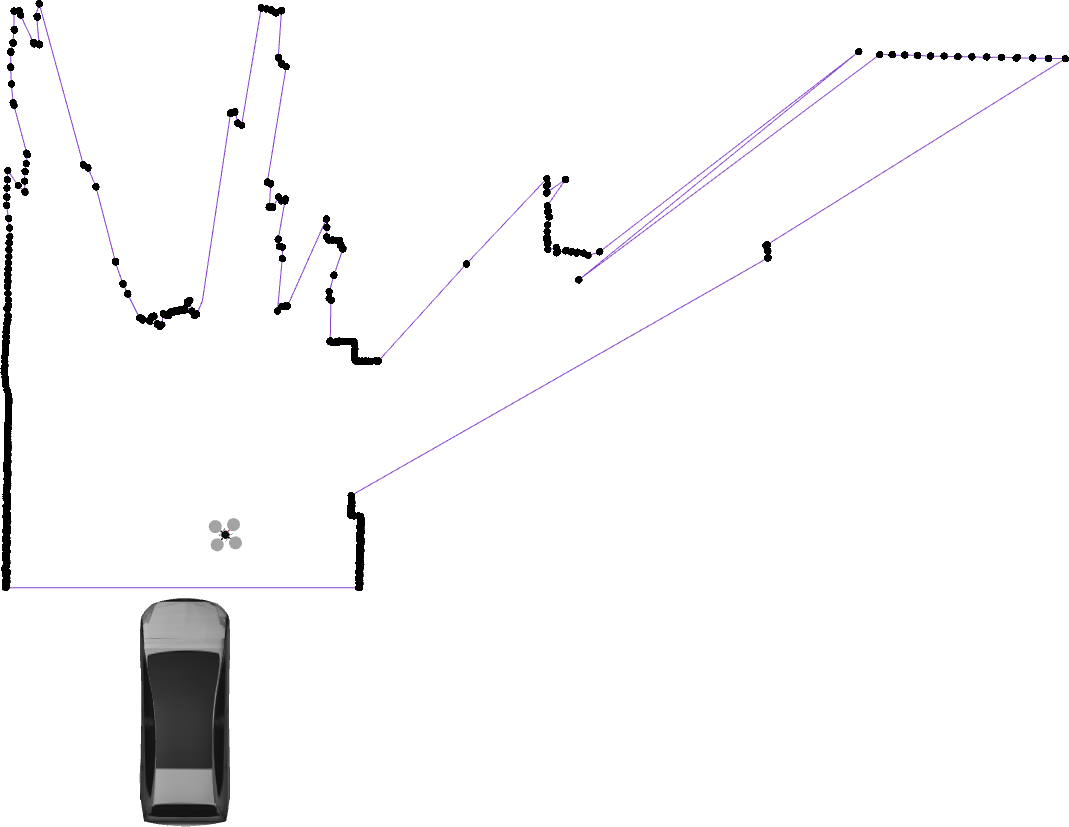
\includegraphics[width=0.49\linewidth]{02polygon} \\
%     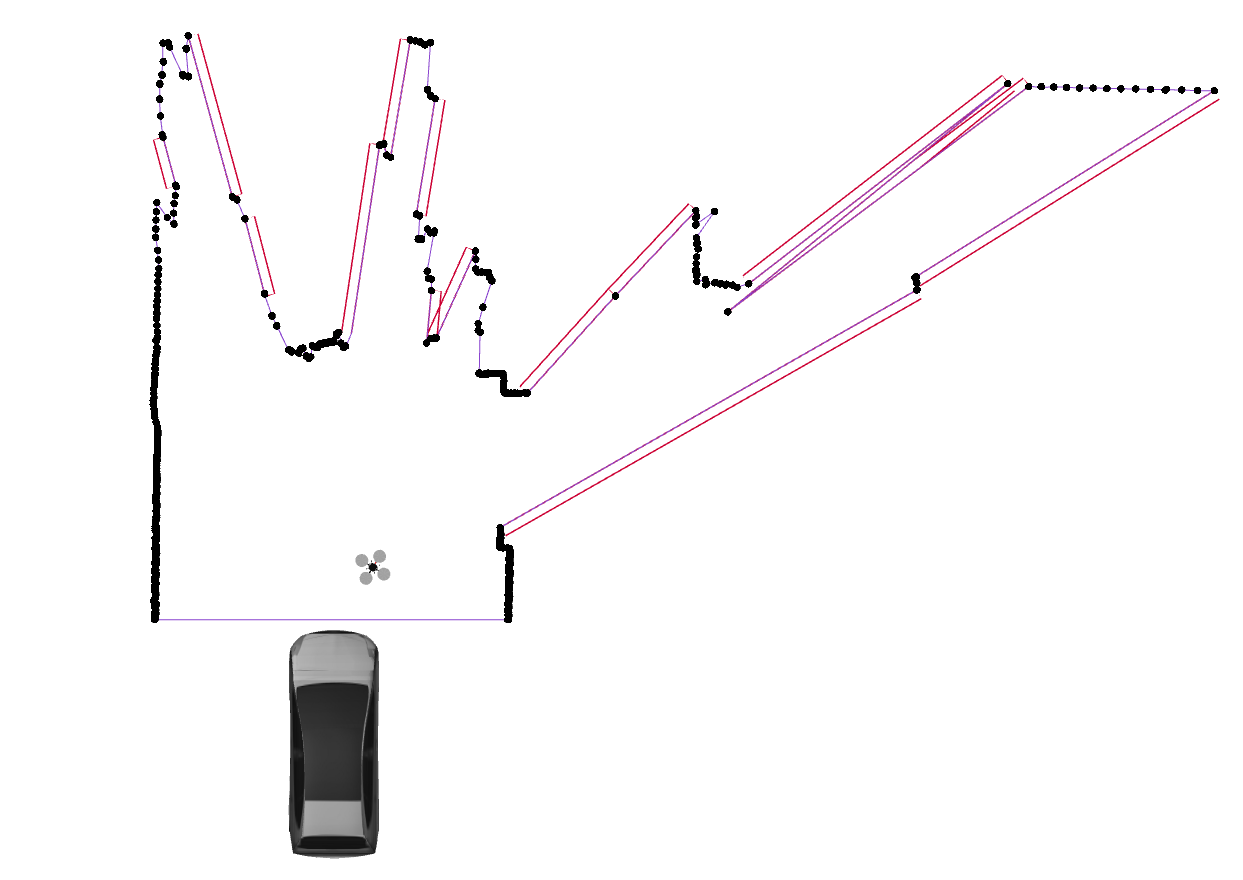
\includegraphics[width=0.49\linewidth]{03blindspots}
%     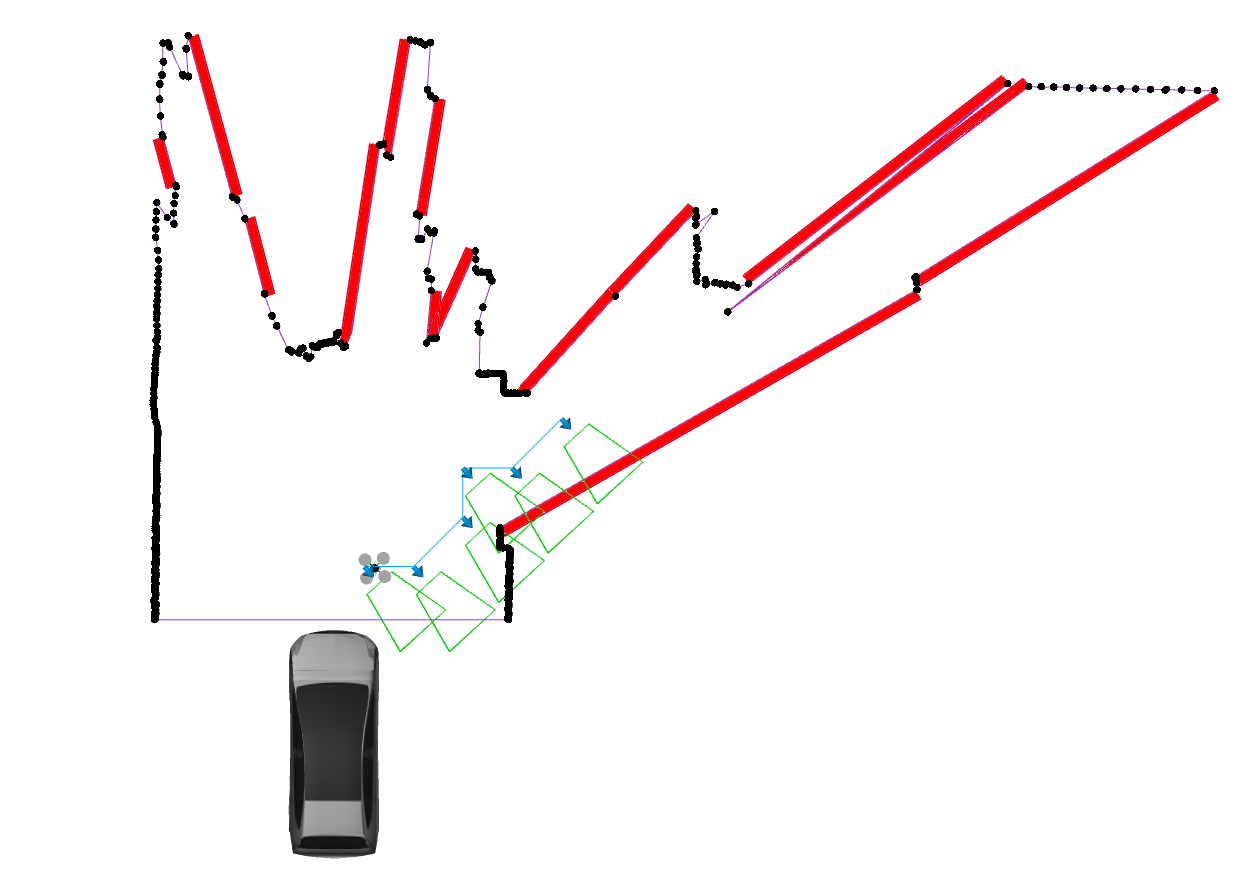
\includegraphics[width=0.49\linewidth]{04planner}
% \end{figure}

\subsection{Finding the Bounding Polygon}

\label{sec:poly}

The bounding polygon computed using a scan from the 2D LiDAR sensor on the car
is used as a conservative representation of the free space in which the
quadrotor can travel. Below we provide a formal definition of a laser scan that
is used in the rest of the paper.

\begin{definition}

    A laser scan is a sequence of points, $L = \{\mathbf{c} + r_i \cdot [\cos
    \theta_i, \sin \theta_i] ^ T : \theta_{\min} \leq \theta_i \leq
    \theta_{\max} \} \subset \R^2$, where $\mathbf{c}$ is the 2D position of
    the LiDAR sensor, $r_i$ is the distance from the sensor to the closest
    obstruction in the $\theta_i$ direction, and
    $[\theta_{\min}$, $\theta_{\max}]$ is the angular range of the sensor.

\end{definition}

From the laser scan, we can easily produce a bounding polygon. The bounding
polygon is defined as the minimum area simple polygon that contains all the
points in the laser scan. Since the laser scan data is ordered by $\theta_i$
from $\theta_{\min}$ to $\theta_{\max}$, the bounding polygon can be
constructed in one pass with the vertex sequence $\{\mathbf{c}\} \cup L \cup
\{\mathbf{c}\}$. Fig.~\ref{fig:polygon} shows an example of laser scan
data and the corresponding bounding polygon.

\begin{figure}[ht]

    \centering
    % 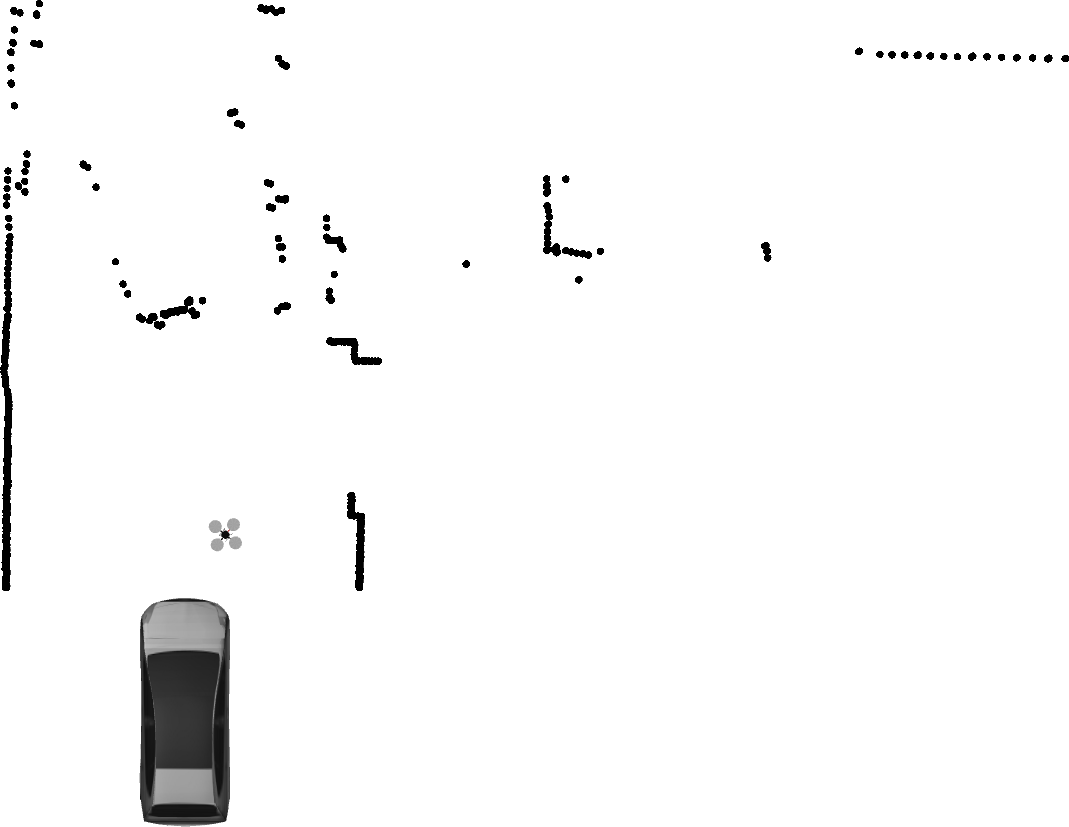
\includegraphics[width=0.49\linewidth]{01laser}
    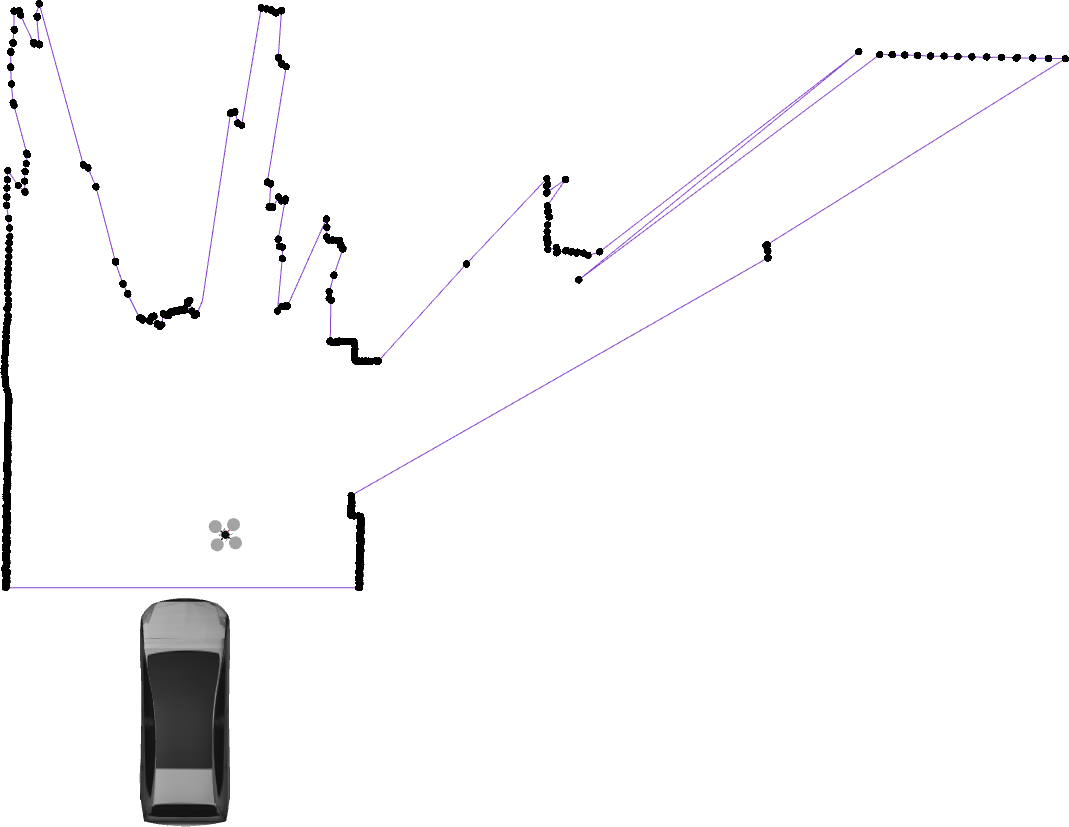
\includegraphics[width=1\linewidth]{02polygon}
    % 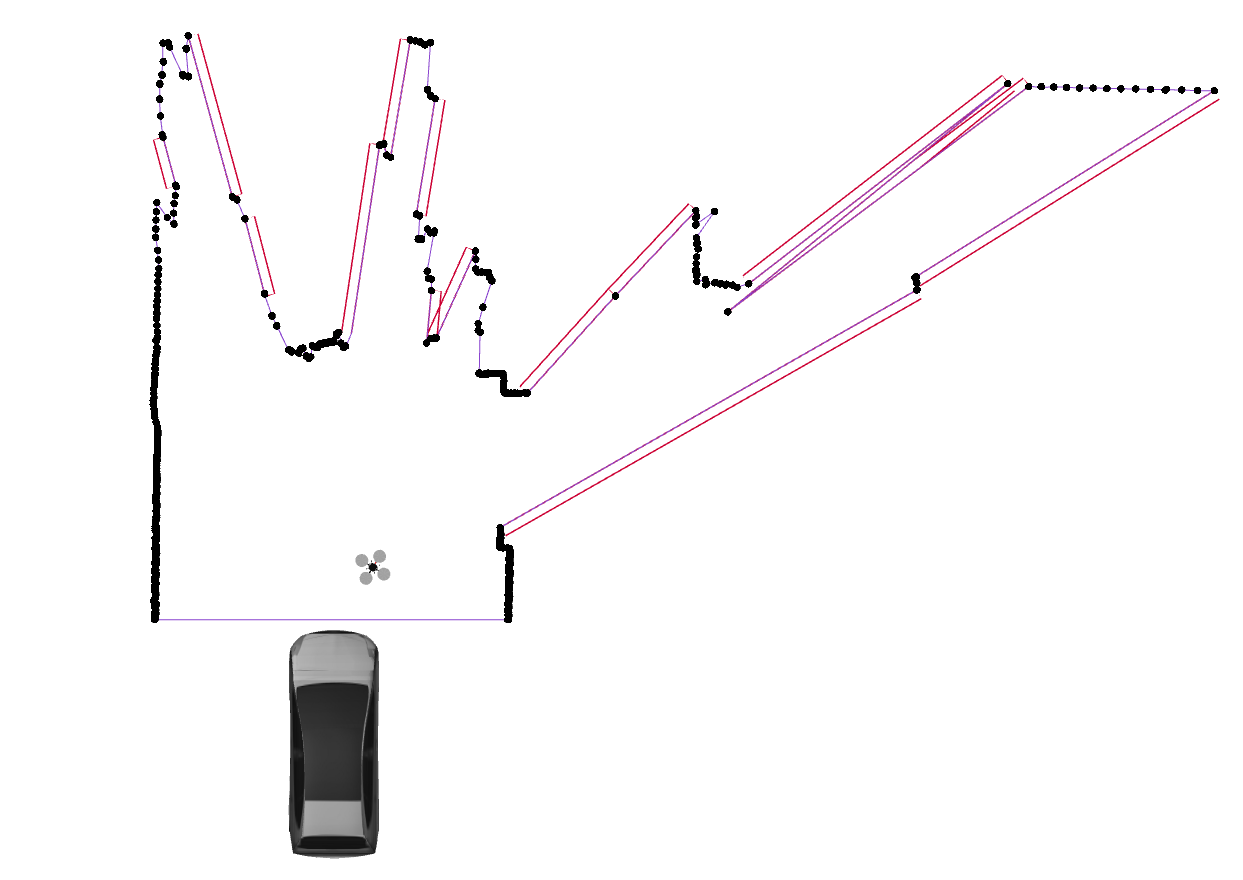
\includegraphics[width=0.49\linewidth]{03blindspots}
    % 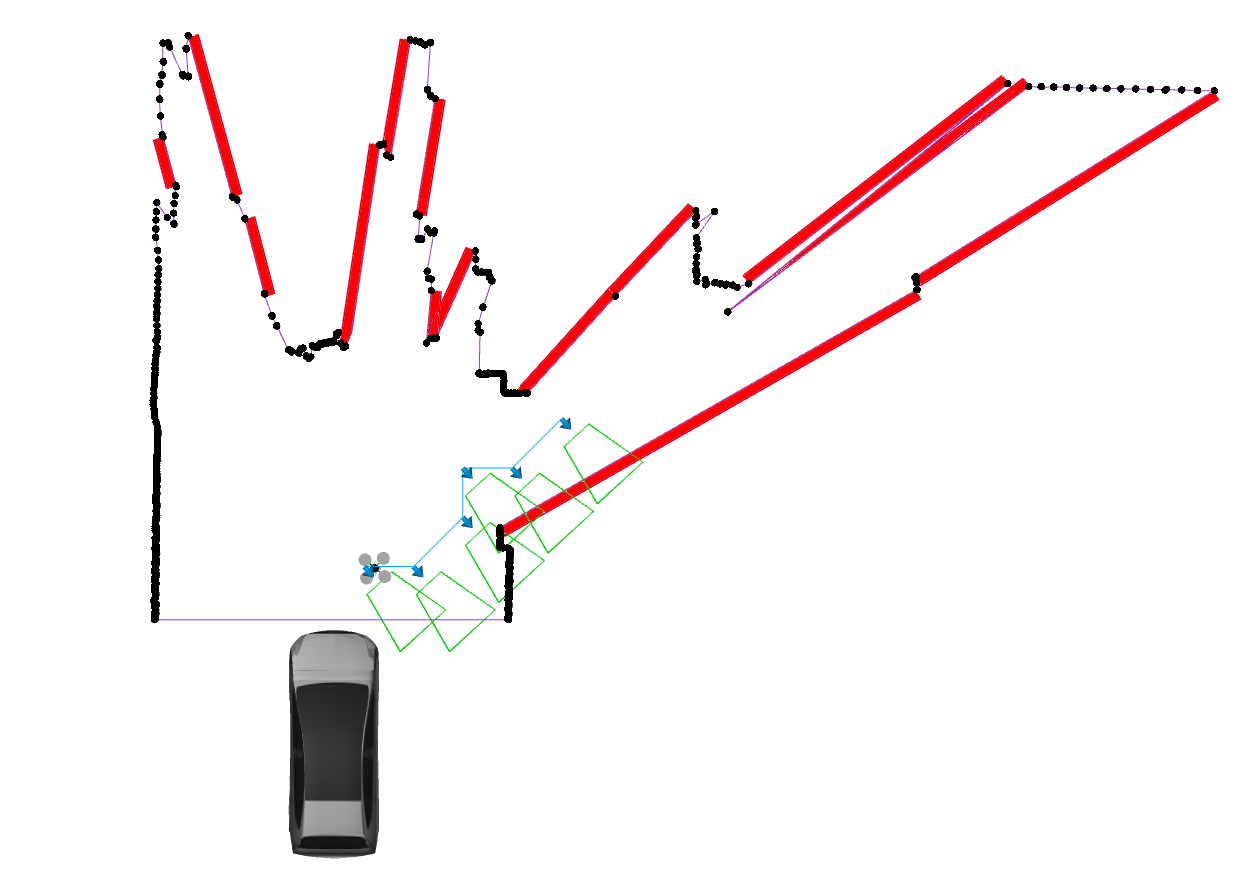
\includegraphics[width=0.49\linewidth]{04planner}

    \caption{Constructing the bounding polygon from the laser scan. The black
        circles are the individual points in the scan and the purple lines
        are the line segments in the bounding polygon.}

    \label{fig:polygon}
\end{figure}

\subsection{Determining the Blind Regions}

\label{sec:blindregions}

Using the laser scan data, we can determine which areas in the environment the
car is unable to sense. We call these areas blind regions. The blind region is
a rectangle, $B$, with a vertex sequence $\{L_i, L_i + k \cdot \hat{L}_{i, i +
1}, L_{i + 1} + k \cdot \hat{L}_{i, i + 1}, L_{i + 1}, L_i\}$ where
$\hat{L}_{i, i + 1}$ is the unit normal for the vector between points $L_i$ and
$L_{i + 1}$ that points away from the bounding polygon and $k$ is a tuning
parameter that contributes to the area of the blind region. In practice we only
care for blind regions where $||L_i - L_{i + 1}||_2 > \delta$ where $\delta$ is
a tuning parameter. We will use $\B$ to denote the set of all such regions.
Fig.~\ref{fig:blindregions} shows an example of blind regions in found in a
found from a laser scan.

\begin{figure}[ht]

    \centering
    % 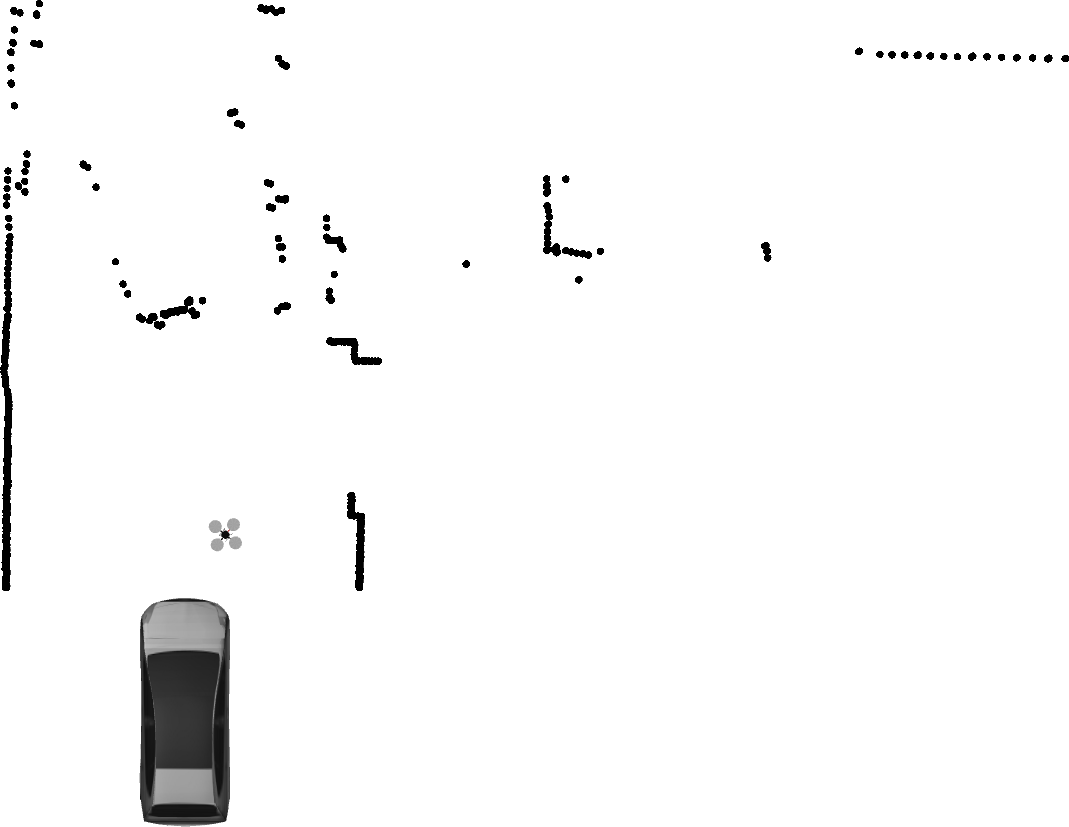
\includegraphics[width=0.49\linewidth]{01laser}
    % 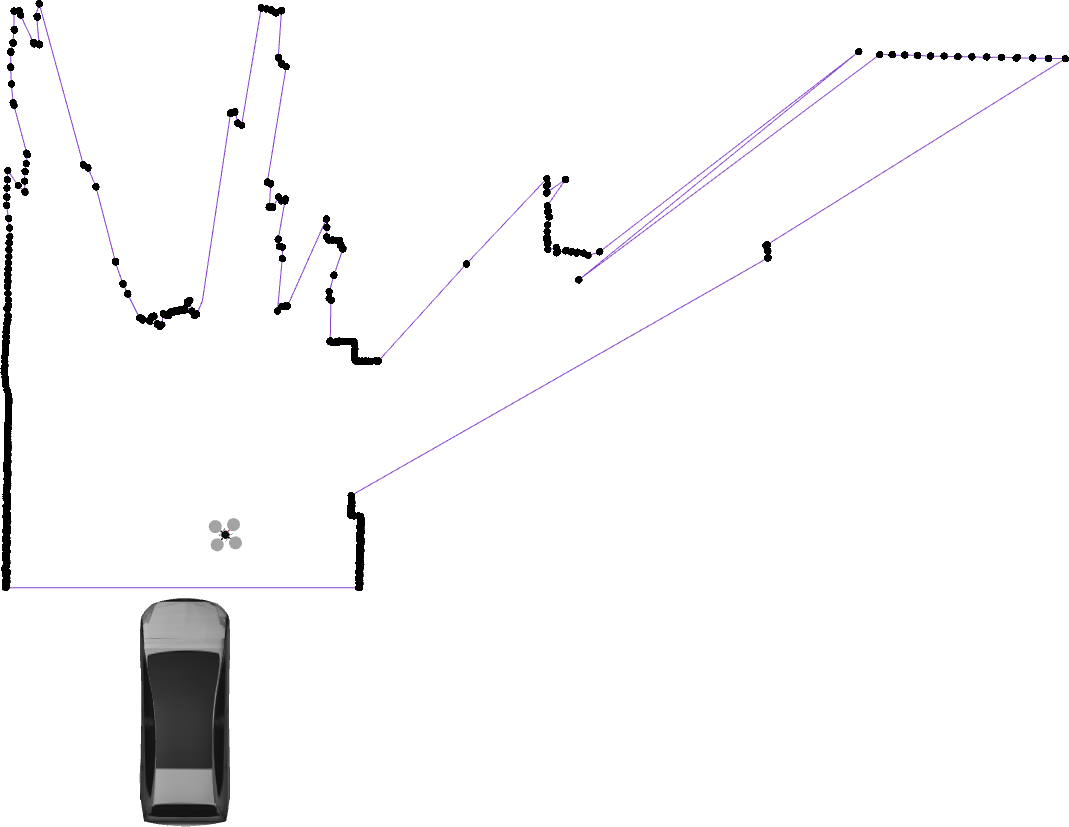
\includegraphics[width=1\linewidth]{02polygon}
    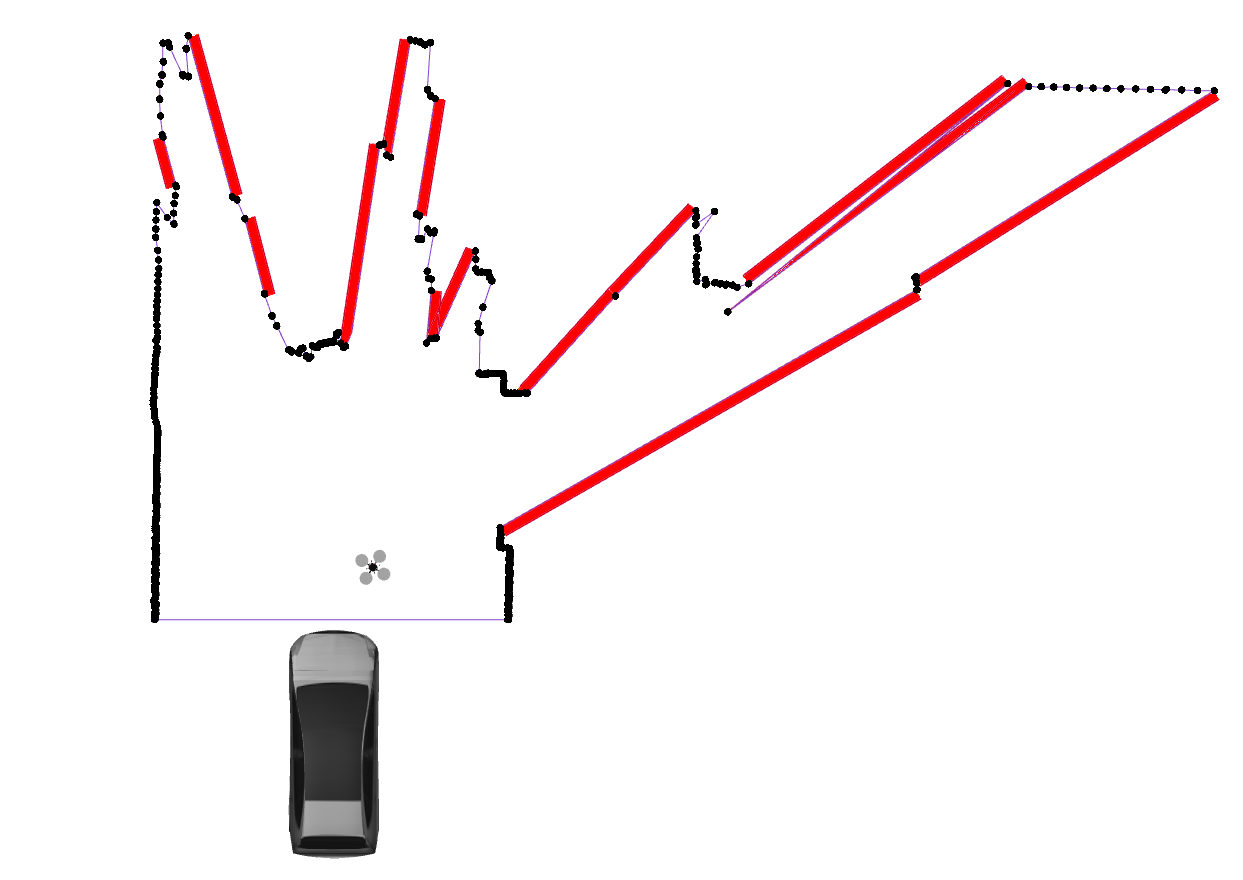
\includegraphics[width=1\linewidth]{03blindregions}
    % 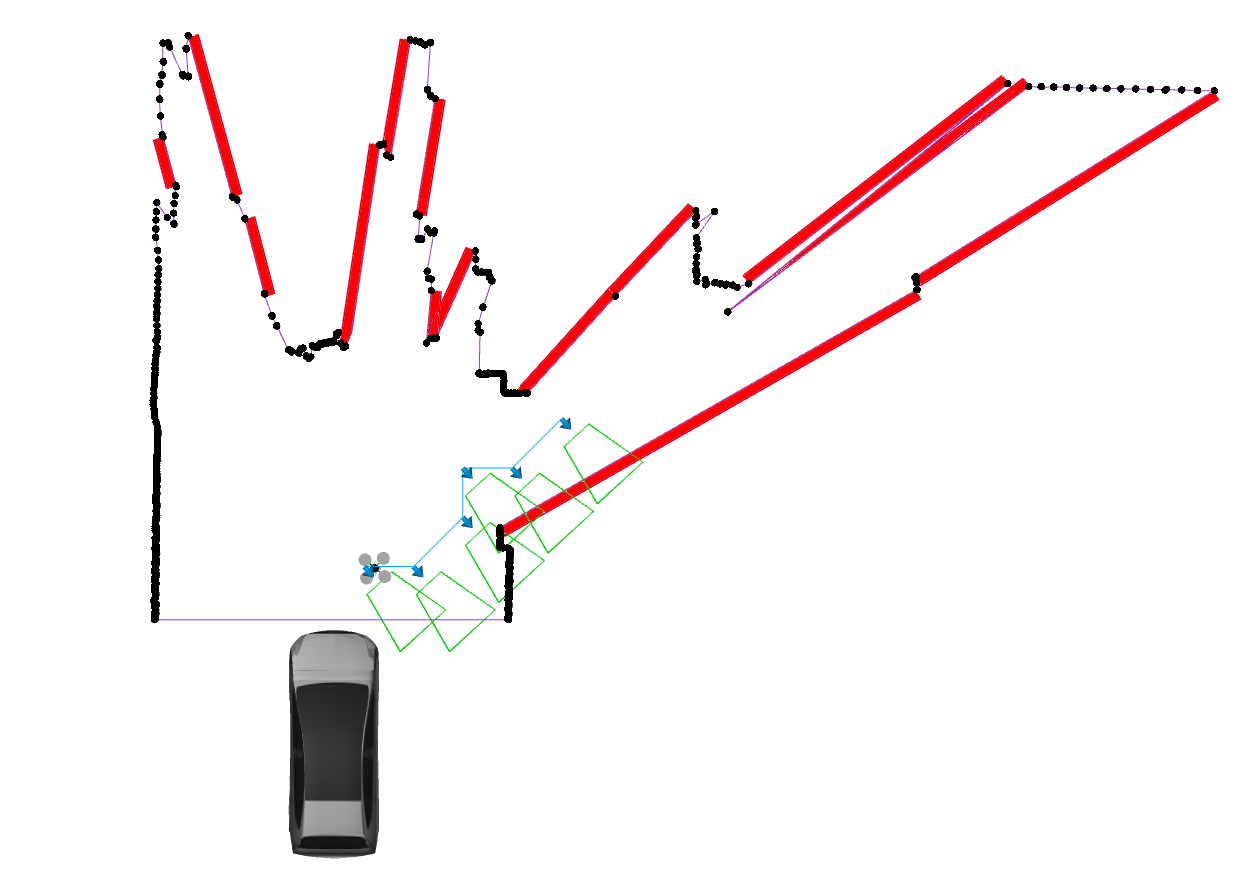
\includegraphics[width=0.49\linewidth]{04planner}

    \caption{Finding the blind regions from the laser scan. The black circles
        are individual points in the scan and the red filled rectangles are the
        blind regions}

    \label{fig:blindregions}
\end{figure}

% maybe can change the name of this section
\subsection{Computing the Exploratory Path}

\label{sec:planner}

Using the blind regions, current configuration of the quadrotor, and the
bounding polygon, we present an anytime algorithm that computes a collision
free path for the quadrotor that maximizes the total observed area of the blind
regions within a given time horizon. The algorithm builds a search tree
starting from the current configuration of the quadrotor. It expands leaf nodes
in descending order of total observed blind region area and only adds new leaf
nodes to the search that are contained within the bounding polygon. As the
quadrotor follows the path, the planner is constantly replanning. To avoid
oscillating between candidate paths, the quadrotor only follows a new path if
its current path is no longer collision free or if the new path has a larger
objective value. Algo.~\ref{algo:find_path} formally describes how the path is
computed.

\begin{algorithm}[h!]
    \caption{Algorithm caption}
    \algorithmicrequire{\begin{itemize}
            \item $x_0$: The initial position of the robot
            \item $\B$: The blind region
        \end{itemize}}
    \algorithmicensure{\begin{itemize}
            \item $\Pi \subset \R^3 \times [0, 2\pi]$: A sequence of 3D positions
                and orientations representing the path
        \end{itemize}}
    \label{algo:find_path}
    \begin{algorithmic}[1]
        \setcounter{ALC@line}{0}
        % \vspace*{1mm}

        \STATE $Q \leftarrow \{(x_0, \phi^*(x_0, \B),
            \B \, \backslash \, \psi^*(x_0, \B))\}$
        \WHILE{$|Q| > 0$}

        \STATE $(x, \theta, \rB) \leftarrow \argmin{\rB \in Q} \Area(\rB)$

            \IF{$\Function{SearchTimeoutExpired}()$}
                \STATE $\Pi \leftarrow \{\}$
                \WHILE{$\Function{HasParent}(x, \theta)$}
                    \STATE $\Pi \leftarrow \Pi \cup \{x\}$
                    \STATE $(x, \theta) \leftarrow \Function{Parent}(x, \theta)$
                \ENDWHILE
                \RETURN $\Pi$
            \ENDIF
            \FORALL{$x' \in \Function{CollisionFreeNeighbours}(x)$}
            \STATE $\theta' \leftarrow \phi^*(x', \rB)$
            \STATE $Q \leftarrow Q \cup \{(x', \theta', \rB \, \backslash \,
                    \psi^*(x', \rB))\}$
                \STATE $\Function{Parent}(x', \theta') \leftarrow (x, \theta)$
            \ENDFOR
            \STATE $Q \leftarrow Q \, \backslash \, \{(x, \phi, \rB)\}$
        \ENDWHILE
        \RETURN $\{\}$

    \end{algorithmic}
\end{algorithm}

At the start of Algo.~\ref{algo:find_path}, we initialize a priority queue that
is used to store the leaf nodes in the search tree. Each node is comprised of
the position of the quadrotor, $x \in \R^3$, the orientation of the quadrotor
on the Z-axis, $\theta \in [0, 2\pi]$, and the remaining blind region, $\B$,
that is left unobserved after the quadrotor reaches $x$ with orientation
$\theta$. The function $\phi^*(x, \B)$ returns the orientation for $x \in
\R^3$ that maximizes the area of the blind region $\B$ that is observed.
Similarly, the function $\psi^*(x, \B)$ returns the set of points that the
camera is able to observe from $x$, if it had orientation, $\phi^*(x, \B)$.

% \begin{definition}
%
%     A laser scan is a sequence of points, $L \subset \R^2$, such that
%     if a polygon, $P$, is constructed with these points, there exists a point,
%     $c \in \R^2$, such that $\forall x \in L$, the line segment from
%     $c$ to $x$ is entirely contained in $P$.
%
% \end{definition}
%
% \begin{definition}
%
%     A break in the laser scan is a line segment $(L_i, L_{i + 1})$ such that
%     $||L_i - L_{i + 1}||_2 > \delta$ where $\delta$ is the break threshold. The
%     set of all these breaks will be referred to as $\tilde L$.
%
% \end{definition}
%
% \begin{definition}
%
%     A blind spot, $B(L_i, L_{i + 1})$, is the set of points contained between
%     the line segments, $(L_i, L_{i + 1})$ and $(L_i + \epsilon \cdot \hat n,
%     L_{i + 1} + \epsilon \cdot \hat n)$ where $\hat n$ is the unit normal of
%     the line segment $(L_i, L_{i + 1})$, $\epsilon$ is a parameter governing
%     the size of the region, and $(L_i, L_{i + 1})$ is a break in the laser
%     scan.
%
% \end{definition}
%
% \begin{definition}
%
%     The blind region, $\mathcal{B}$, for a laser scan, $L$, is defined as
%     $\mathcal{B} = \bigcup_{(i, j) \in \tilde L} B(i, j)$.
%
% \end{definition}
%
% \begin{definition}
%
%     The sensor projection for our robot, $\psi(x, \theta)$ is defined as the
%     set of points that the robot is able to observe from configuration $x$ with
%     yaw, $\theta$. The optimal sensor projection for a given configuration and
%     blind region is defined as $\psi^*(x, \B) = \psi(x, \theta^*(x, \B))$ with
%     $\theta^*(x, \B) = \argmax{0 < \theta \leq 2\pi} \Area(\B \cap \psi(x,
%     \theta))$
%
% \end{definition}
%
% \begin{definition}
%
%     A path, $\rho \subset V \times [0, 2 \pi]$, is a sequence of tuples, $(x,
%     \theta)$, consisting of state and yaw, such that $\forall
%     i : (\rho_{i, x}, \rho_{i + 1, x}) \in E$, where $G = (V, E)$ is a finite
%     sampled graph within the polygon constructed using the laser scan, $L$,
%     that represents the connectivity of the free space.
%
% \end{definition}
%
% \begin{algorithm}[h!]
%     \caption{}
%     \algorithmicrequire{\begin{itemize}
%             \item $x_0$: The initial position of the robot
%             \item $\B$: The blind region
%             \item $G = (V, E)$: The finite sampled graph within the laser scan
%                 polygon
%             \item $\gamma$, $C$: The optimality and cumulative cost thresholds
%                 respectively for the algorithm's termination
%         \end{itemize}}
%     \algorithmicensure{\begin{itemize}
%             \item $\rho \subset V \times [0, 2\pi]$: A sequence of tuples
%                 representing the path
%         \end{itemize}}
%     \label{algo:find_path}
%     \begin{algorithmic}[1]
%         \setcounter{ALC@line}{0}
%         \vspace*{1mm}
%
%         \STATE $Q \leftarrow \{(x_0, \B \, \backslash \, \psi^*(x_0, \B), 0)\}$
%         \WHILE{$|Q| > 0$}
%             \STATE $(x, \rB, c) \leftarrow \argmin{q \in Q} \Area(q_{\rB})$
%             \IF{$\Area(\B \, \backslash \, \rB) > \gamma \cdot \Area(\B)$}
%                 \STATE $\rho \leftarrow \{\}, \, \hat x \leftarrow x', \,
%                     \hat \B \leftarrow \rB, \, \hat c \leftarrow c$
%                 \WHILE{$\Function{HasParent}(\hat x, \hat B, \hat c)$}
%                     \STATE $\rho \leftarrow \{(\hat x,
%                         \theta^*(\hat x, \hat \B))\} \cup \rho$
%                     \STATE $(\hat x, \hat \B, \hat c) \leftarrow
%                         \Function{Parent}(\hat x, \hat \B, \hat c)$
%                 \ENDWHILE
%                 \RETURN $\rho$
%             \ENDIF
%             \FORALL{$x' \where (x, x') \in E$}
%                 \STATE $c' \leftarrow c + \Function{CostToGo}(x, x')$
%                 \IF{$c' < C$}
%                     \STATE $Q \leftarrow Q \cup \{(x', \rB \, \backslash \,
%                         \psi^*(x', \rB), c')\}$
%                     \STATE $\Function{Parent}(x', \rB \, \backslash \,
%                         \psi^*(x', \rB), c') \leftarrow (x, \rB, c)$
%                 \ENDIF
%             \ENDFOR
%             \STATE $Q \leftarrow Q \, \backslash \, (x, \rB, c)$
%         \ENDWHILE
%         \RETURN $\False$
%
%     \end{algorithmic}
% \end{algorithm}
%
% \begin{lemma}
%
%     \label{lemma:cost}
%
%     If a path is returned from Algo.~\ref{algo:find_path}, it will have a total
%     cost less than $C$.
%
% \end{lemma}
%
% \begin{proof}
%
%     At each iteration, the cost to reach each neighbour of $x$ is computed.
%     This is added to the total cost of current path. If the cost of the path
%     from $x_0$ to $x'$ is larger than $C$, it is discarded from the search.
%     Thus only path with cost less than $C$, can be returned from
%     Algo.~\ref{algo:find_path}.
%
% \end{proof}
%
% \begin{lemma}
%
%     \label{lemma:finite}
%
%     Algo.~\ref{algo:find_path} will finish in a finite number of steps if
%     $\forall (i, j) \in E: \Function{CostToGo}(i, j) \geq 1$ and $C < \infty$
%
% \end{lemma}
%
% \begin{proof}
%
%     Since the cumulative cost being added to search is monotonically
%     increasing, if a given path is not returned, its cost will eventually be
%     greater than $C$ in a finite amount of time since, $C <
%     \infty$ and all individual costs must be greater than 1. If no path is
%     returned by the algorithm, it means that all paths in $G$ have not reached
%     the optimality threshold with their costs being less than $C$. Since $G$ is
%     a finite graph, there are a finite amount of paths and therefore, to
%     determine if no path will be returned takes a finite number of steps. If a
%     path is returned, Algo.~\ref{algo:find_path} is returning the first path
%     that meets the optimality threshold which would occur before all paths in G
%     are exhausted, thus returning in a finite number of steps.
%
% \end{proof}
%
% \begin{lemma}
%
%     \label{lemma:res_area}
%
%     At each iteration, the residual blind region, $\B_n = \B \, \backslash \,
%     \bigcup\limits_{(x_i, \theta_i) \in \rho} \psi(x_i, \theta_i)$ where $\rho$
%     is the path from $x_0$ to $x_n$.
%
% \end{lemma}
%
% \begin{proof}
%
%     At the $n^{\text{th}}$, the blind region in the tuple being added to $Q$ is
%
%     \begin{align*}
%         \B_n = \B \, \backslash \, \psi^*(x_0, \B) \, \backslash \,
%         \psi^*(x_1, \B_0)
%         \backslash \ldots \backslash \psi^*(x_n, \B_{n - 1})
%     \end{align*}
%
%     where $\B_i$ is the residual blind region for the $i^{\text{th}}$ step in
%     path. Now we can rearrange to produce
%
%     \begin{align*}
%         \B_n = \B \, \backslash \, \bigcup_{i = 0}^{n - 1}
%         \psi^*(x_i, \B_{i - 1}) \\
%     \end{align*}
%
%     Now since $\psi^*(x_i, \B_{i - 1}) =
%     \psi(x_i, \theta^*(x_i, \B_{i - 1})) = \psi(x_i, \theta_i)$, because
%     the optimal yaw is added to the path for a given residual blind region,
%
%     \begin{align*}
%         \B_n = \B \, \backslash \bigcup_{(x_i, \theta_i) \in \rho}
%         \psi(x_i, \theta_i)
%     \end{align*}
%
% \end{proof}
%
% \begin{theorem}
%
%     If there exists a path, $\rho$, such that $\Function{Area}(\mathcal{B}
%     \, \cap \, \bigcup_{(x, \theta) \in \rho} \psi(x, \theta)) >  \gamma \cdot
%     \Function{Area}(\mathcal{B})$ and $\rho$ can be executed by the
%     robot with a total cost less than $C$, Algo.~\ref{algo:find_path} will
%     return such a path in a finite number of steps.
%
% \end{theorem}
%
% \begin{proof}
%
%     Using Lemmas~\ref{lemma:cost} and~\ref{lemma:finite}, we know that any path
%     returned from Algo.~\ref{algo:find_path} will have a total cost less than
%     $C$ and it will be returned in a finite number steps.  We also know from
%     Lemma~\ref{lemma:res_area}, that the blind region at the $n^{\text{th}}$
%     iteration is $\B \, \backslash
%         \bigcup_{(x_i,
%             \theta_i) \in
%     \rho} \psi(x_i, \theta_i)$. Now, note that,
%
%     \begin{align*}
%         \B \backslash \B_n &= \B \backslash (\B \, \backslash
%         \bigcup_{(x_i, \theta_i) \in \rho} \psi(x_i, \theta_i)) \\
%         &= \B \cap
%         \bigcup_{(x_i, \theta_i) \in \rho} \psi(x_i, \theta_i)
%     \end{align*}
%
%     Now since, the algorithm only returns a path if $\Area(\B \backslash
%     \B_n) > \gamma \cdot \Area(\B)$ and using the result above, the algorithm
%     will only return a path such that $\Area(\B \cap
%     \bigcup_{(x_i, \theta_i) \in \rho} \psi(x_i, \theta_i)) >
%     \gamma \cdot \Area(\B)$
% \end{proof}
